\documentclass[a4paper,10pt]{article}
\usepackage[utf8]{inputenc}
\usepackage[english]{babel}
\usepackage{geometry}
\usepackage[T1]{fontenc}
\usepackage{float}
\usepackage{multirow}
\usepackage{booktabs}
\usepackage{chemfig}
\usepackage{amsmath}
\usepackage{xcolor}
\usepackage{pxfonts}
\usepackage{tikz}

\title{DSL Tutorial}
\author{}



\newcommand{\gerquot}[1]{\glqq#1\grqq}
\newcommand{\dashAndSpace}{\textendash \space}
\newcommand{\dashAndSpaceSeq}[1]{\dashAndSpace#1 \textendash}

\newcommand{\DSL}{domain specific language}
\newcommand{\CFG}{context-free grammar}
\newcommand{\IUPAC}{International Union of Pure and Applied Chemistry}

\newcommand{\captionVSpace}{\vspace*{-0.05cm}}
\newcommand{\connectionThicknessDefault}{1.5pt}
\newcommand{\CFGDefinitionSize}{0.60}
\newcommand{\SymbolDescriptionTable}{0.35}

\newcommand{\colorBracketFirstNesting}{black}
\newcommand{\colorBracketSecondNesting}{blue}
\newcommand{\colorBracketThirdNesting}{green}
\newcommand{\colorBracketFourthNesting}{red}
\newcommand{\colorBracketFifthNesting}{cyan}
\newcommand{\colorBracketSixthNesting}{yellow}
\newcommand{\colorBracketSeventhNesting}{brown}
\newcommand{\colorBracketEigthNesting}{orange}

\newcommand{\colorNew}{orange}
\newcommand{\colorMainChain}{blue}
\newcommand{\colorBranchFirstNesting}{orange}

%%%%% %%%%% %%%%% %%%%% %%%%% %%%%% %%%%% %%%%%                %%%%% %%%%% %%%%% %%%%% %%%%% %%%%% %%%%% %%%%%
%%%%% %%%%% %%%%% %%%%% %%%%% %%%%% %%%%% %%%%% BEGIN document %%%%% %%%%% %%%%% %%%%% %%%%% %%%%% %%%%% %%%%%
%%%%% %%%%% %%%%% %%%%% %%%%% %%%%% %%%%% %%%%%                %%%%% %%%%% %%%%% %%%%% %%%%% %%%%% %%%%% %%%%%
\begin{document}

\maketitle

\section{Motivation}\label{s:Motivation}
To understand technologies like DSLs (\DSL) examples are the best way to explain different aspects, e.g. use cases, typical problems, limitations, etc. Instead of creating an artificial example, in general a real world instance offers an more plain view to a technology.

Because of this reason the IUPAC naming system as an example was chosen. Maybe you already heard this name from the school in the chemistry subject. For those, who did not have any idea about this naming system or for people without any chemical background knowledge, don't worry; \emph{this tutorial focuses on the naming system itself} and has only low contact points to the chemical background.

The goal is to make a tutorial, that explains the creation of CFG (\CFG) and illustrate the differences of abstract syntax and concrete syntax. We do not expect, that you are a expert in this topic; but a basic knowledge should be available. Terms like \gerquot{grammar} or \gerquot{production rule} will not be explained.



\section{History of the IUPAC naming convention}\label{s:HistoryOfTheIUPACNamingConvention}
At be beginning some history. IUPAC is an abbreviation for \emph{\IUPAC}. This union was founded in 1919 with the goal to simplify the global communication between chemists. Up to this year no global rules were available for naming chemical structures. Every country used his own system and this leaded to many misunderstandings; sometimes even in a single country. You can compare this situation like before the metric system was invented.

The IUPAC invented a systematic way to create a unique name for \dashAndSpaceSeq{in theory} every chemical structure. In most cases the literature uses the term \gerquot{IUPAC name} or \gerquot{IUPAC nomenclature} for a name in the IUPAC convention. In this tutorial both of this terms will be also used.

The rules of this naming convention can be formulated as \CFG. So it can be also understood as a kind of DSL. In the following sections basic rules of the naming convention will be introduced. And also the way to cast it to a \CFG.



\section{Introduction to the IUPAC nomenclature}\label{s:IntroductionToTheIUPACNomenclature}
Carbon (C) has the unique skill to create long structures with branches and nesting, that are stable \dashAndSpace in a chemical point of view. The possibilities are tremendous. Almost all other elements are not capable of creating larger structures. So the naming convention focuses on the carbon and the describing of that structures.

\subsection{Nothing than straight chains}\label{ss:NothingThanStraightChains}
In a simplified manner you can compare a carbon atom with a building block: The simplest way is a straight chain of carbon atoms without any branches. The IUPAC nomenclature encodes the length of such a straight chain in specific terms like \gerquot{Methan}, \gerquot{Ethan}, etc. See the table \ref{tab:NumCarbonEncodedName} below for a length up to 10 carbon atoms.

\begin{table}[H]
    \centering
    \begin{tabular}{c|l}
        \toprule
        \textbf{Number of carbon atoms} & \textbf{Encoded name} \\
        \midrule
        1 & Methan \\
        2 & Ethan \\
        3 & Propan \\
        4 & Butan \\
        5 & Pentan \\
        6 & Hexan \\
        7 & Heptan \\
        8 & Octan \\
        9 & Nonan \\
        10 & Decan \\
        \bottomrule
    \end{tabular}
    \captionVSpace
    \caption{List of the first 10 names for a straight chain}
    \label{tab:NumCarbonEncodedName}
\end{table}

\noindent For example: \\
\emph{Ethan}\qquad
\setchemfig{chemfig style={line width=\connectionThicknessDefault}}
\chemfig{C-C} \\
or \\
\emph{Hexan}\qquad
\setchemfig{chemfig style={line width=\connectionThicknessDefault}}
\chemfig{C-C-C-C-C-C} \\

In a sense of a grammar: This term for the straight chain is the main symbol. We call this symbol $c$ (for chain). $S$ is our mandatory start symbol and thus it is a nonterminal symbol. For this tutorial $T$ the set for terminal symbols; $N$ for nonterminal and $P$ for all production rules are used. In summary our first CFG grammar has the following definition:

\begin{figure}[H]
    \begin{minipage}[l]{\CFGDefinitionSize\textwidth}
        $$
        \begin{aligned}
            T &=& \{c\} \\
            N &=& \{S\} \\
            P &:& \\
            S &\rightarrow& c \\
        \end{aligned}
        $$
        \caption{The CFG with only straight chains.}
        \label{fig:CFGOnlyStraightChains}
    \end{minipage}
    \begin{minipage}[r]{\SymbolDescriptionTable\textwidth}
        \begin{table}[H]
        \centering
            \begin{tabular}{c|l}
                \toprule
                \textbf{Symbol} & \textbf{Description} \\
                \midrule
                c & Main chain \\
                \bottomrule
            \end{tabular}
            %\captionVSpace
            %\caption{Descriptions of the terminal symbols}
        \end{table}
    \end{minipage}
\end{figure}


\subsection{First order branches}\label{ss:FirstOrderBranches}
A chain of carbon atoms can also contain branches. This branches could also be nested; for now we focus on branches without deeper nesting. To identify a branch we need the length of this branch and the position. The position will be formulated from the point of view of the main chain. The length of the branch will be encoded in terms. These terms are comparable with the terms for the main chain but with a postfix \gerquot{yl} instead of \gerquot{an}. This are the first 5 terms for the encoded branch length:

\begin{table}[H]
    \centering
    \begin{tabular}{c|l}
        \toprule
        \textbf{Number of carbon atoms in branch} & \textbf{Encoded name} \\
        \midrule
        1 & Methyl \\
        2 & Ethyl \\
        3 & Propyl \\
        4 & Butyl \\
        5 & Pentyl \\
        ... & ... \\
        \bottomrule
    \end{tabular}
    \captionVSpace
    \caption{List of the first 5 names for a branch}
    \label{tab:NumCarbonBranchEncodedName}
\end{table}

\noindent An example for this: \\
\begin{figure}[H]
    \centering
    \setchemfig{chemfig style={line width=\connectionThicknessDefault}}
    \chemfig{C-[,,,,\colorMainChain]C(-[6,,,,\colorBranchFirstNesting]C)-[,,,,\colorMainChain]C-[,,,,\colorMainChain]C-[,,,,\colorMainChain]C-[,,,,\colorMainChain]C-[,,,,\colorMainChain]C} \\
    \caption{Example with one branch of the length 1}
    \label{fig:SecondExample}
\end{figure}
The orange one is the branch with the length of one C atom. So the name is \emph{Methyl}. Any position information is written in front of the corresponding branch with a minus char between them. The full branch is therefore: \emph{2-Methyl}. The main chain has the length 7 $\rightarrow$ \emph{Heptan}.

So we can see, that a branch with the position information consists of three parts:
\begin{itemize}
    \item Position $p \in \mathbb{N}$
    \item Minus sign $m$
    \item Term for the length of the branch $b$
\end{itemize}
Because every branch has this structure, we can introduce a nonterminal symbol to summarize all three terminals in this symbol $B$.

What about the order of branches and main chain? The IUPAC convention defines, that the term for the main chain will be always at the end of the name. This is good for the CFG definition, because we don't need to add production rules for both orders. With this and the other new information we have now following grammar (new elements are highlighted):

\begin{figure}[H]
    \begin{minipage}[l]{\CFGDefinitionSize\textwidth}
        $$
        \begin{aligned}
            T &=& \{c, {\color{\colorNew}p, m, b}\} \\
            N &=& \{S, {\color{\colorNew}B, M}\} \\
            P &:& \\
            S &\rightarrow& {\color{\colorNew}M} \\
            {\color{\colorNew}M} &\rightarrow& {\color{\colorNew}Bc} \\
            {\color{\colorNew}M} &\rightarrow& {\color{\colorNew}c} \\
            {\color{\colorNew}{B}} &\rightarrow& {\color{\colorNew}pmb} \\
        \end{aligned}
        $$
        \caption{CFG with exact one branch. $B \rightarrow pmb$ is an optional production rule.}
        \label{fig:CFGWithExactOneBranch}
    \end{minipage}
    \begin{minipage}[r]{\SymbolDescriptionTable\textwidth}
        \begin{table}[H]
        \centering
            \begin{tabular}{c|l}
                \toprule
                \textbf{Symbol} & \textbf{Description} \\
                \midrule
                c & Main chain \\
                p & position \\
                m & minus char \\
                b & branch \\
                \bottomrule
            \end{tabular}
            %\captionVSpace
            %\caption{Descriptions of the terminal symbols}
        \end{table}
    \end{minipage}
\end{figure}

It is important to notice, that an additional nonterminal ($M$) was added. Because a grammar can only contains exact one start variable, we need $M$ as \gerquot{middle variable} to make words with and without branches possible. In summary: the $B$ is \dashAndSpaceSeq{like a branch} an optional nonterminal.
The whole name of the structure in figure \ref{fig:SecondExample} is: \emph{2-MethylHeptan}\footnote{It can produced with
$
S
{\color{\colorBracketFirstNesting}{(}}
    M
    {\color{\colorBracketSecondNesting}{(}}
        B
        {\color{\colorBracketThirdNesting}{(}}
            pmb
        {\color{\colorBracketThirdNesting}{)}}
        , c
    {\color{\colorBracketSecondNesting}{)}}
{\color{\colorBracketFirstNesting}{)}}
$}

\subsection{Multiple first order branches}\label{ss:MultipleFirstOrderBranches}
No one can forbid the carbon atoms to create multiple branches of the same length. Let add an another branch of the length one at the third position:
\begin{figure}[H]
    \centering
    \setchemfig{chemfig style={line width=\connectionThicknessDefault}}
    \chemfig{C-[,,,,\colorMainChain]C(-[6,,,,\colorBranchFirstNesting]C)-[,,,,\colorMainChain]C(-[6,,,,\colorBranchFirstNesting]C)-[,,,,\colorMainChain]C-[,,,,\colorMainChain]C-[,,,,\colorMainChain]C-[,,,,\colorMainChain]C} \\
    \caption{Example with two branches of the length 1}
    \label{fig:ThirdExample}
\end{figure}

The intuitive way is to assume, that a second branch with the new position will be added to the begin of the name. It would be understandable; but it increases the name and in many molecules 5 to 10 branches and sometimes more are usual. For this reason there is a prefix to summarize branches of the same length. Table \ref{tab:BranchesWithTheSameLength} shows the first 5 prefixes.

\begin{table}[H]
    \centering
    \begin{tabular}{c|l}
        \toprule
        \textbf{Branches with the same length} & \textbf{Prefix} \\
        \midrule
        1 & Mono \\
        2 & Di \\
        3 & Tri \\
        4 & Tetra \\
        5 & Penta \\
        \bottomrule
    \end{tabular}
    \captionVSpace
    \caption{List of the first 5 prefixes to summarize branches with the same length}
    \label{tab:BranchesWithTheSameLength}
\end{table}

In normal cases the prefix \gerquot{Mono} is not used. So in the name \emph{1-MethylHeptan} is no \gerquot{Mono} missing!\footnote{The nomenclature defines no specific rules for the usage. So for this tutorial \gerquot{Mono} will be not used.}

To identify also the second brach, we need the position of them. All position information will be written before the branch term and the prefix to summarize branches with the same length before the correspondig branch term: \emph{2,3-DiMethylHeptan}. Usually the positions are sorted in ascending order. Between two numbers a comma is added to avoid ambiguous meanings if the positions larger than 9.

To formulate this in a grammar we have the situation, that position numbers can occur multiple times on the same branch term. So at least one production rule for branches needs to create a non-terminal symbol. We can isolate the parts for the position information from the symbol $B \rightarrow pmb$ in a new symbol $C$. $p$ ans $m$ will be moved to $C$, so that $C$ is $C \rightarrow pm$. A second $C$, that creates itself, is necessary for multiple position information. This second $C$ could be: $C \rightarrow poC$ ($o$ represents here the comma char). \emph{Or in more simple words: we need to define production rules, they can create itself to make loops possible.}

With the prefix, that summarizes multiple branches (we call it $d$), we have a similar situation like with $M$. This prefix $d$ is an optional symbol, so we need an additional production rule to achive this. An additional $B$ seems to be a good choice.

\begin{figure}[H]
    \begin{minipage}[l]{\CFGDefinitionSize\textwidth}
        $$
        \begin{aligned}
            T &=& \{c, p, m, b, {\color{\colorNew}o, d}\} \\
            N &=& \{S, B, M, {\color{\colorNew}C}\} \\
            P &:& \\
            S &\rightarrow& M \\
            M &\rightarrow& Bc \\
            M &\rightarrow& c \\
            % {\color{\colorNew}M} &\rightarrow& {\color{\colorNew}C} \\
            {\color{\colorNew}B} &\rightarrow& {\color{\colorNew}C} \\
            {\color{\colorNew}C} &\rightarrow& {\color{\colorNew}pmb} \\
            {\color{\colorNew}C} &\rightarrow& {\color{\colorNew}poC} \\
            {\color{\colorNew}C} &\rightarrow& {\color{\colorNew}mdb} \\
        \end{aligned}
        $$
        \caption{CFG with multiple branches and same length. Several usage of $C \rightarrow poC$ creates successive positions.}
        \label{fig:CFGWithMultipleBranchesAtTheSameLength}
    \end{minipage}
    \begin{minipage}[r]{\SymbolDescriptionTable\textwidth}
        \begin{table}[H]
        \centering
            \begin{tabular}{c|l}
                \toprule
                \textbf{Symbol} & \textbf{Description} \\
                \midrule
                c & Main chain \\
                p & position \\
                m & minus char \\
                b & branch \\
                o & comma char \\
                d & summary prefix \\
                \bottomrule
            \end{tabular}
            %\captionVSpace
            %\caption{Descriptions of the terminal symbols}
        \end{table}
    \end{minipage}
\end{figure}

\noindent The word \emph{2,3-DiMethylHeptan} can be produced with:
$
S
{\color{\colorBracketFirstNesting}{(}}
    M
    {\color{\colorBracketSecondNesting}{(}}
        C
        {\color{\colorBracketThirdNesting}{(}}
            po,
            C
            {\color{\colorBracketFourthNesting}{(}}
                po,
                C
                {\color{\colorBracketFifthNesting}{(}}
                    mdb
                {\color{\colorBracketFifthNesting}{)}}
            {\color{\colorBracketFourthNesting}{)}}
        {\color{\colorBracketThirdNesting}{)}}
        , c
    {\color{\colorBracketSecondNesting}{)}}
{\color{\colorBracketFirstNesting}{)}}
$\\


In theory we have the grammar, which fulfills the requirements. But look at the production:
$
S
{\color{\colorBracketFirstNesting}{(}}
    M
    {\color{\colorBracketSecondNesting}{(}}
        B
        {\color{\colorBracketThirdNesting}{(}}
            C
            {\color{\colorBracketFourthNesting}{(}}
                mdb
            {\color{\colorBracketFourthNesting}{)}}
        {\color{\colorBracketThirdNesting}{)}}
        , c
    {\color{\colorBracketSecondNesting}{)}}
{\color{\colorBracketFirstNesting}{)}}
$
It creates the word $\textbf{mdbc}$. A word with a minus char, a prefix like \gerquot{Tri}, a branch and the name for the main chain like \gerquot{Hexan}. E.g.: \emph{-TriMethylHexan}. Such a word makes no sense. So the grammer is too open. We describe more words than wanted. The reason for this is, that $C$ contains multiple different productions; only with sense, if there are used in a specific order. This is a hint for missing nonterminal symbols. A generic $C$ is also too simple.\\

\noindent One problem are the positon information. We have here two different scenarios:
\begin{itemize}
    \item One singe position with a minus sign; E.g. \emph{2-}
    \item Multiple position information separated with a comma and with a minus sign at the end. E.g. \emph{2,3,4-}
\end{itemize}
We cannot gurantee with our current approach, that a summary prefix will be followed, if we have multiple position information. For example: \emph{2,3,4-Methyl...} is in our grammer although the summary prefix \emph{Tri} is missing. The reason is, that we here focused only on the position information and we have no way to influence the using of the summary prefix. The is an recurring problem with loops in a grammer when the number of used loops influence part of the words outside of the loop content. The figure \ref{fig:OldStyleMultiplePositions} shows the situation with the current $P$.

\begin{figure}[H]
\centering
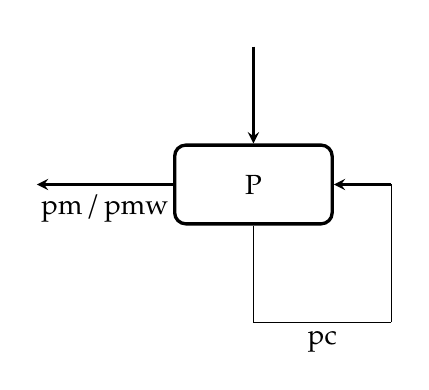
\begin{tikzpicture}[node distance=1.75cm]
    \tikzstyle{in_out} = [rectangle, rounded corners, minimum width=2cm, minimum height=1cm, text centered, draw=black, very thick]%, fill=red!30]
    \tikzstyle{rect} = [rectangle, rounded corners, minimum width=3cm, minimum height=1cm, text centered, draw=black]
    \tikzstyle{process} = [rectangle, rounded corners, minimum width=0.75cm, minimum height=0.75cm,text centered, draw=black, fill=gray!12.5]
    \tikzstyle{intersection} = [rectangle, rounded corners, minimum width=4cm, minimum height=1cm, text centered, draw=black]
    \tikzstyle{arrow} = [thick,->,>=stealth]

    \node (InputP) [in_out, xshift=0cm] {P};

    \node (InvIn) [coordinate, above of=InputP, xshift=0cm, yshift=-0cm, label=] {};
    \node (InvOut) [coordinate, left of=InputP, xshift=-1cm, yshift=-0cm, label=] {};

    \node (Inv1) [coordinate, below of=InputP, xshift=0cm, yshift=-0cm, label=] {};
    \node (Inv2) [coordinate, right of=Inv1, xshift=0cm, yshift=-0cm, label=] {};
    \node (Inv3) [coordinate, above of=Inv2, xshift=0cm, yshift=-0cm, label=] {};

    % ----- ----- ----- ----- ----- ----- ----- ----- ----- ----- ----- ----- ----- ----- ----- ----- ----- ----- -----

    \draw [arrow] (InvIn) -- node[anchor=east] {} (InputP);

    \draw (InputP) -- node[anchor=east] {} (Inv1);
    \draw (Inv1) -- node[anchor=north] {pc} (Inv2);
    \draw (Inv2) -- node[anchor=east] {} (Inv3);
    \draw [arrow] (Inv3) -- node[anchor=east] {} (InputP);

    \draw [arrow] (InputP) -- node[anchor=north] {pm / pmw} (InvOut);
\end{tikzpicture}
\caption{$P$ can produce itself. $pmw$ should only created, when at least one time $P$ created itself.}
\label{fig:OldStyleMultiplePositions}
\end{figure}

$P$ can create correct words. But it cannot determine, whether at least one time $P$ created itself. So all words \dashAndSpaceSeq{with and without} summary prefix can be created. In a programming language we could use a flag or something similar. In a CFG this approach is not usable, because we don't have variables, that can be altered. The only possibility to solve this issue is to introduce a new nonterminal \dashAndSpace here called $P_2$. For the sake of completeness we rename $P$ to $P_1$.\\

$P_2$ can only be reached, if at least one times $pc$ was produced. So the usage of the nonterminal $P_2$ itself holds the information, that a summary prefix must be used. Figure \ref{fig:NewStyleMultiplePositions} shows the modified visualization of $P$.

\begin{figure}[H]
\centering
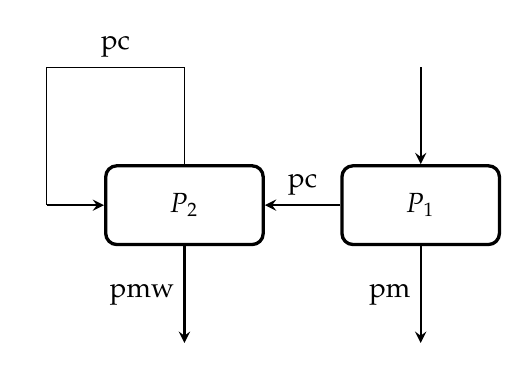
\begin{tikzpicture}[node distance=1.75cm]
    \tikzstyle{in_out} = [rectangle, rounded corners, minimum width=2cm, minimum height=1cm, text centered, draw=black, very thick]%, fill=red!30]
    \tikzstyle{rect} = [rectangle, rounded corners, minimum width=3cm, minimum height=1cm, text centered, draw=black]
    \tikzstyle{process} = [rectangle, rounded corners, minimum width=0.75cm, minimum height=0.75cm,text centered, draw=black, fill=gray!12.5]
    \tikzstyle{intersection} = [rectangle, rounded corners, minimum width=4cm, minimum height=1cm, text centered, draw=black]
    \tikzstyle{arrow} = [thick,->,>=stealth]

    \node (InputP1) [in_out, xshift=0cm] {$P_1$};
    \node (InputP2) [in_out, xshift=-3cm] {$P_2$};

    \node (InvIn) [coordinate, above of=InputP1, xshift=0cm, yshift=-0cm, label=] {};
    \node (InvOut2) [coordinate, below of=InputP2, xshift=0cm, yshift=-0cm, label=] {};
    \node (InvOut1) [coordinate, below of=InputP1, xshift=0cm, yshift=-0cm, label=] {};

    \node (Inv1) [coordinate, above of=InputP2, xshift=0cm, yshift=-0cm, label=] {};
    \node (Inv2) [coordinate, left of=Inv1, xshift=0cm, yshift=-0cm, label=] {};
    \node (Inv3) [coordinate, below of=Inv2, xshift=0cm, yshift=-0cm, label=] {};

    % ----- ----- ----- ----- ----- ----- ----- ----- ----- ----- ----- ----- ----- ----- ----- ----- ----- ----- -----

    \draw [arrow] (InvIn) -- node[anchor=east] {} (InputP1);
    \draw [arrow] (InputP1) -- node[anchor=east] {pm} (InvOut1);

    % P1 -> P2
    \draw [arrow] (InputP1) -- node[anchor=south] {pc} (InputP2);

    \draw (InputP2) -- node[anchor=east] {} (Inv1);
    \draw (Inv1) -- node[anchor=south] {pc} (Inv2);
    \draw (Inv2) -- node[anchor=east] {} (Inv3);
    \draw [arrow] (Inv3) -- node[anchor=east] {} (InputP2);
    \draw [arrow] (InputP2) -- node[anchor=east] {pmw} (InvOut2);
\end{tikzpicture}
\caption{Modified $P$. The usage of $P_2$ gurantees, that at least one times $pm$ was created.}
\label{fig:NewStyleMultiplePositions}
\end{figure}

\begin{figure}[H]
    \begin{minipage}[l]{\CFGDefinitionSize\textwidth}
        $$
        \begin{aligned}
            T &=& \{c, p, m, b, o, d\} \\
            N &=& \{S, M, {\color{\colorNew}P_1, P_2}\} \\
            P &:& \\
            S &\rightarrow& M \\
            M &\rightarrow& {\color{\colorNew}P_1}c \\
            M &\rightarrow& c \\
            % {\color{\colorNew}M} &\rightarrow& {\color{\colorNew}C} \\
            {\color{\colorNew}P_1} &\rightarrow& {\color{\colorNew}pmb} \\
            {\color{\colorNew}P_1} &\rightarrow& {\color{\colorNew}poP_2} \\
            {\color{\colorNew}P_2} &\rightarrow& {\color{\colorNew}poP_2} \\
            {\color{\colorNew}P_2} &\rightarrow& {\color{\colorNew}pmdb} \\
        \end{aligned}
        $$
        \caption{Adjusted CFG with $P_1$ and $P_2$.}
        \label{fig:CFGWithMultipleBranchesAtTheSameLengthNewApproach}
    \end{minipage}
    \begin{minipage}[r]{\SymbolDescriptionTable\textwidth}
        \begin{table}[H]
        \centering
            \begin{tabular}{c|l}
                \toprule
                \textbf{Symbol} & \textbf{Description} \\
                \midrule
                c & Main chain \\
                p & position \\
                m & minus char \\
                b & branch \\
                o & comma char \\
                d & summary prefix \\
                \bottomrule
            \end{tabular}
            %\captionVSpace
            %\caption{Descriptions of the terminal symbols}
        \end{table}
    \end{minipage}
\end{figure}

We see, that our grammar uses now complete new production rules. One noticeable change are the production rules $P_1$ and $P_2$ with the same result $poP_2$. This is an usual way to define loops in a CFG. With the altered CFG, the production of \emph{2,3-DiMethylHeptan} is also modified:
$
S
{\color{\colorBracketFirstNesting}{(}}
    M
    {\color{\colorBracketSecondNesting}{(}}
        P_1
        {\color{\colorBracketThirdNesting}{(}}
            po,
            P_2
            {\color{\colorBracketFourthNesting}{(}}
                pmdb
            {\color{\colorBracketFourthNesting}{)}}
        {\color{\colorBracketThirdNesting}{)}}
        , c
    {\color{\colorBracketSecondNesting}{)}}
{\color{\colorBracketFirstNesting}{)}}
$.



\section{Abstract- and Concrete Syntax Trees}\label{s:AbstractAndConcreteSyntaxTrees}
In the section \ref{s:IntroductionToTheIUPACNomenclature} we used the tupel description of the CFG. In the tupel description every detail of the language is defined. And the production even of a simple word contains multiple nested parentheses. Already with a few production rules, the grammer becomes complex to handle and especially to debug (see chapter \ref{ss:MultipleFirstOrderBranches}).

% For this reason the syntax tree was invented. This is a more graphical way to describe a grammer. And the abstract syntax tree foucuses on the structural details instead of describing the whole formal language.


\end{document}
%%%%% %%%%% %%%%% %%%%% %%%%% %%%%% %%%%% %%%%%              %%%%% %%%%% %%%%% %%%%% %%%%% %%%%% %%%%% %%%%%
%%%%% %%%%% %%%%% %%%%% %%%%% %%%%% %%%%% %%%%% END document %%%%% %%%%% %%%%% %%%%% %%%%% %%%%% %%%%% %%%%%
%%%%% %%%%% %%%%% %%%%% %%%%% %%%%% %%%%% %%%%%              %%%%% %%%%% %%%%% %%%%% %%%%% %%%%% %%%%% %%%%%
